\documentclass[12pt,a4paper]{article}
\usepackage[margin=2cm]{geometry}
\usepackage{titling}
\usepackage{graphicx}
\usepackage{subcaption}
\setlength{\droptitle}{-5em} 
\usepackage{algorithm} 
\usepackage{algpseudocode}
\usepackage{enumerate}
\usepackage{float}


\begin{document}
\title{\huge \textbf{Overall Software Plan} \\ \LARGE {\textbf{CS 346: Assignment-2A}}}
\author{\Large Academic Section Management Software}
\date{Group 10A : \texttt{210101113-210101119}}
\maketitle


\section{Problem Statement and Stakeholders}
The project aims to develop a comprehensive academic management software solution for the institute. The system will enable users to perform their assigned tasks efficiently. Key functionalities will include Admissions and Registration, Course Management (including timetable generation), and Examination Management.

\subsubsection*{Stakeholders:}
\begin{itemize}
    \item \textbf{Admin(Dean, Registrar, Administrators):} Responsible for course management and oversight of financial records.
    \item \textbf{Faculty:} Responsible for accessing student information and managing courses, including grading.
    \item \textbf{Students:} Responsible for accessing course information and academic services, as well as submitting fees.
\end{itemize}

\section{Software Model}
The adoption of the \textbf{Structured Analysis and Design} (SAD) model for the development of this specific software is justified by the intricate design and the comprehensive requirements that demand careful consideration. This report documents the different components of this model, including the \textit{Data Dictionary} (encompassing Requirements and Assumptions), \textit{Data Flow Diagrams} (DFDs), and \textit{Entity-Relationship} (E-R) Diagrams in the following sections below.
    

\section{Software Requirements and Assumptions}
The following are the specifications of the software that we are developing as mentioned in the problem statement:
\begin{itemize}
    \item Login details for students and faculties are pre-defined by the Admin. However, they can be changed by the users during the registration process.
    \item We have considered only B.Tech CSE students for timetable generation and examination scheduling processes.
    \item New courses can only be added by the Admin.
    \item Faculty to Course Mapping is done by the Admin itself, and faculties can only access the details of courses that they have been mapped to.
    \item Each course has a unique faculty associated with it, who is responsible for uploading the grades of the enrolled students.
    \item Student Distinction is done only on the basis of their year of study (or semester), ignoring tutorial and lab groups.
    \item The time period for student enrollment, course registration, accessing grades and fee payment are controlled by the Admin.
    \item All lectures have a fixed duration of 1 hour and all labs have a fixed duration of 3 hours.
    \item Lectures are conducted in morning and labs in afternoon for even year and vice-versa for odd year students.
    \item Students can enroll only in courses available during that semester, and can't change them during the semester.
    \item Rooms are of two types: lecture halls and core rooms, and are managed only by the Admin.
    \item Technical support for fee payment is beyond the scope of this software and is only simulated in our system.
\end{itemize}

\section{Data Flow Diagrams}
This section contains a Data Flow Diagram (DFD) to visualize how information flows within the academic management software. It illustrates the movement of data between modules such as Student Enrollment, Course Management, Grade Management, and Examination Management, as well as interactions among stakeholders such as Administrators, Faculty, and Students.

\subsection*{Data flow:}
\begin{itemize}
    \item \textbf{Students} submit enrollment requests, including personal information and desired courses. Approved enrollments are then stored in the system's database.
    \item \textbf{Administrators} publish course schedules, exam timetables, and other academic information.
    \item \textbf{Students} register for the courses they are allowed to enroll in.
    \item \textbf{Students} take exams.
    \item \textbf{Faculty} members update course information and grades as necessary.
\end{itemize}

\subsection{Level-0 DFD}
\begin{figure}[H]
    \centering
        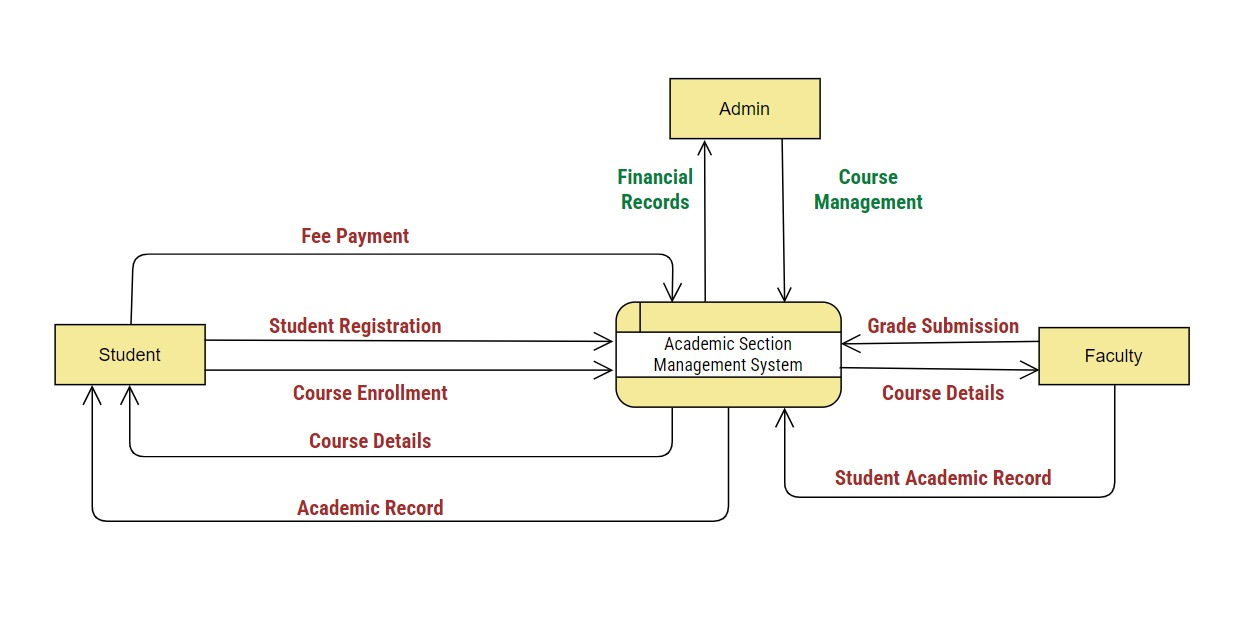
\includegraphics[scale=0.5]{Level_0_DFD.jpg} 
    \caption{\textbf{Level-0 DFD} of our Software.}
\end{figure}
\subsection{Level-1 DFD}
\begin{figure}[H]
    \centering
        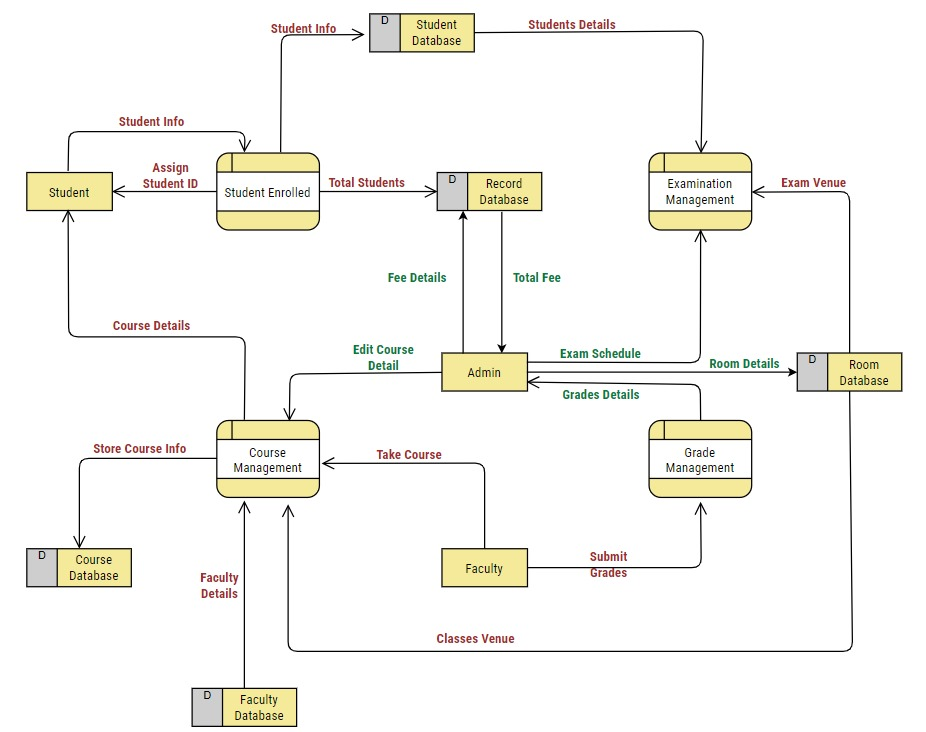
\includegraphics[scale=0.7]{Level_1_DFD.jpg} 
    \caption{\textbf{Level-1 DFD} of our Software.}
\end{figure}


\subsection{Level-2 DFDs}
The following subsections highlight the detailed \textbf{Level-2} Dataflow diagrams of various processes in the Academic system Management software:
\subsubsection{Admission Management Module}
\begin{figure}[H]
    \centering
        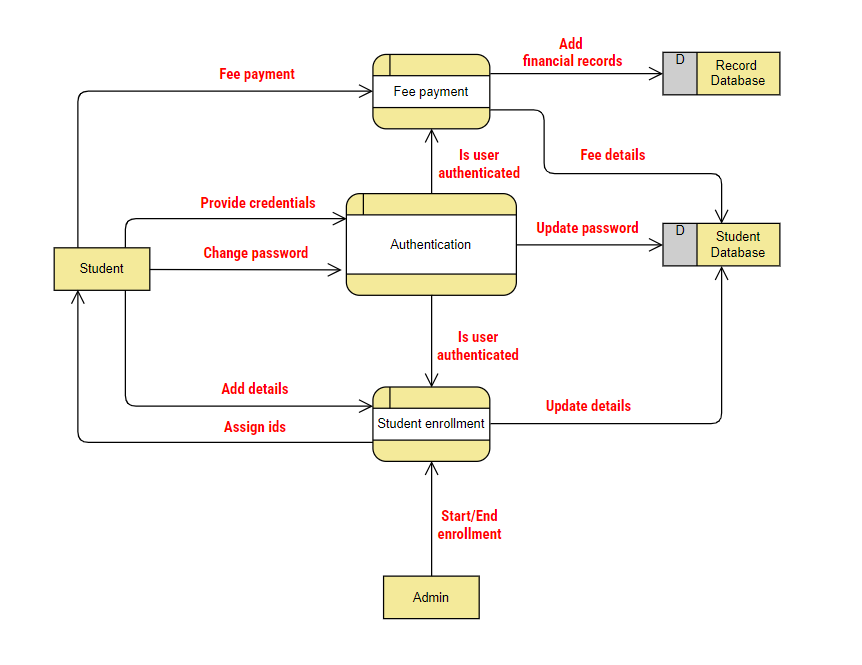
\includegraphics[width=\linewidth]{Student_enrollment_level2_DFD.png} 
    \caption{Level-2 DFD of Admission Management Module}
\end{figure}
\textbf{Admission Management Module} primarily consists of three essential processes :
\begin{enumerate}
	\item \textbf{Authentication} : 
		\begin{itemize}
			\item The Admin configures the password after the JOSAA results and initial username and password is sent to students.
			\item The students can their passwords.
			\item The provided password is then updated in the \textbf{Student Database} for future reference.
		\end{itemize}
	\item \textbf{Student Enrollment} :
		\begin{itemize}
			\item The Admin triggers the course enrollment process.
			\item The students are first checked for authentication.
			\item After that students add their name and year.
			\item Students are then assigned ids.
			\item The details are then added to the \textbf{Student Database}.
		\end{itemize}
	\item \textbf{Fee payment} :
		\begin{itemize}
			\item The students are first authenticated.
			\item Then students pay their fees.
			\item Information about the fees added to \textbf{Student Database}.
			\item These financial records about fees are then added to \textbf{Record Database}.
		\end{itemize}
	
\end{enumerate}

\subsubsection{Course Management Module}
\begin{figure}[H]
    \centering
        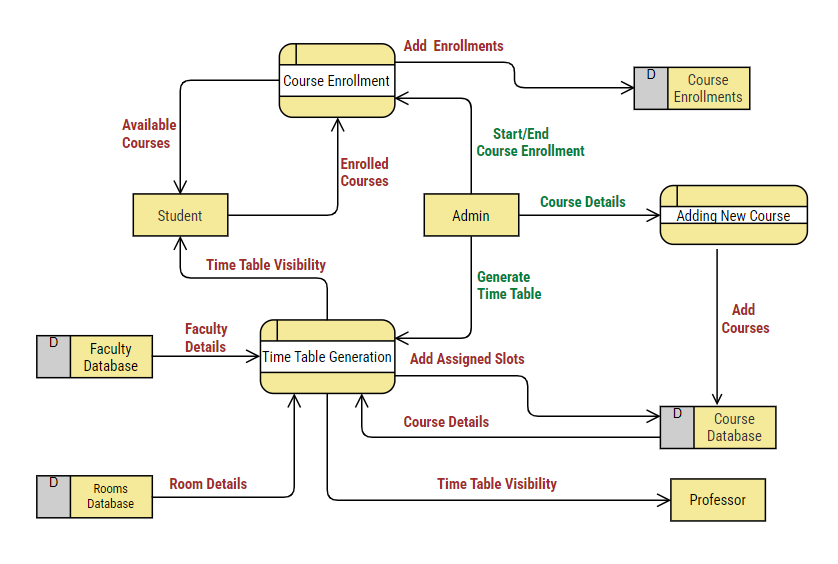
\includegraphics[width=\linewidth]{Course_Management_DFD.png} 
    \caption{Level-2 DFD of Course Management Module}
\end{figure}
\textbf{Course Management Module} primarily consists of three essential processes :
\begin{enumerate}
	\item \textbf{Adding New Course} : 
		\begin{itemize}
			\item The Admin initiates the addition of a new course.
			\item Required details such as course name, credits, valid semesters, and assigned faculty are provided.
			\item The provided course information is then stored in the \textbf{Course Database} for future reference.
		\end{itemize}
	\item \textbf{Course Enrollment} :
		\begin{itemize}
			\item The Admin triggers the course enrollment process.
			\item Students access their interface to view available courses.
			\item Students select a list of courses, including compulsory and department electives.
			\item The selected courses are validated and added to the \textbf{Course Enrollments} database.
		\end{itemize}
	\item \textbf{Time Table Generation} :
		\begin{itemize}
			\item The Admin initiates the time table generation process.
			\item Information from the \textbf{Course Database}, \textbf{Rooms Database}, and \textbf{Faculty Database} is gathered.
			\item The system generates the timetable and modifies the assigned slots in \textbf{Course Database}.
			\item The time table is then displayed on the student and faculty interfaces.
		\end{itemize}
	
\end{enumerate}

\subsubsection{Examination Management Module}
(Pratyush)
\subsubsection{Grade Management Module}
\begin{figure}[H]
    \centering
        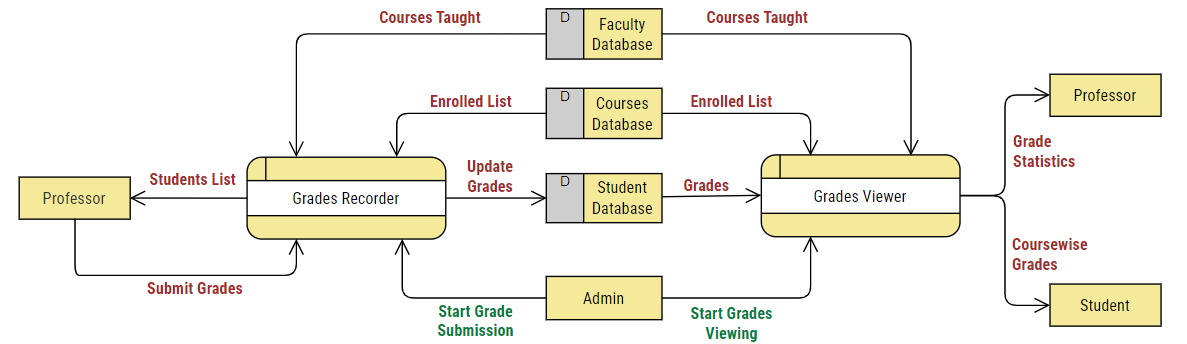
\includegraphics[width=\linewidth]{Grade_Management_DFD.png} 
    \caption{Level-2 DFD of Grade Management Module}
\end{figure}
\begin{itemize}
    \item The \textbf{Grade Recorder} Process first gets the signal from the Admin side to start grade submission.
    \item The professors are displayed the various courses that they teach and they can upload the grade list of students enrolled coursewise, which are updated duly by the Grade Recorder process into \texttt{Grades} field of each course taken by student in \textbf{Student Database}.
    \item The \textbf{Grades Viewer} process first gets the signal from the Admin side after which the students are displayed the grades that they got in specific courses.
    \item The professors can get overall statistics about the grades like Class Average,number of students who got different grades like \texttt{AA,AB,BB} etc.
    \item This particular module interacts with the databases to fetch and update the results, as shown in the DFD diagram of Grade Management module.
\end{itemize}
\section{Entity Relationship Diagram}

\begin{figure}[H]
    \centering
        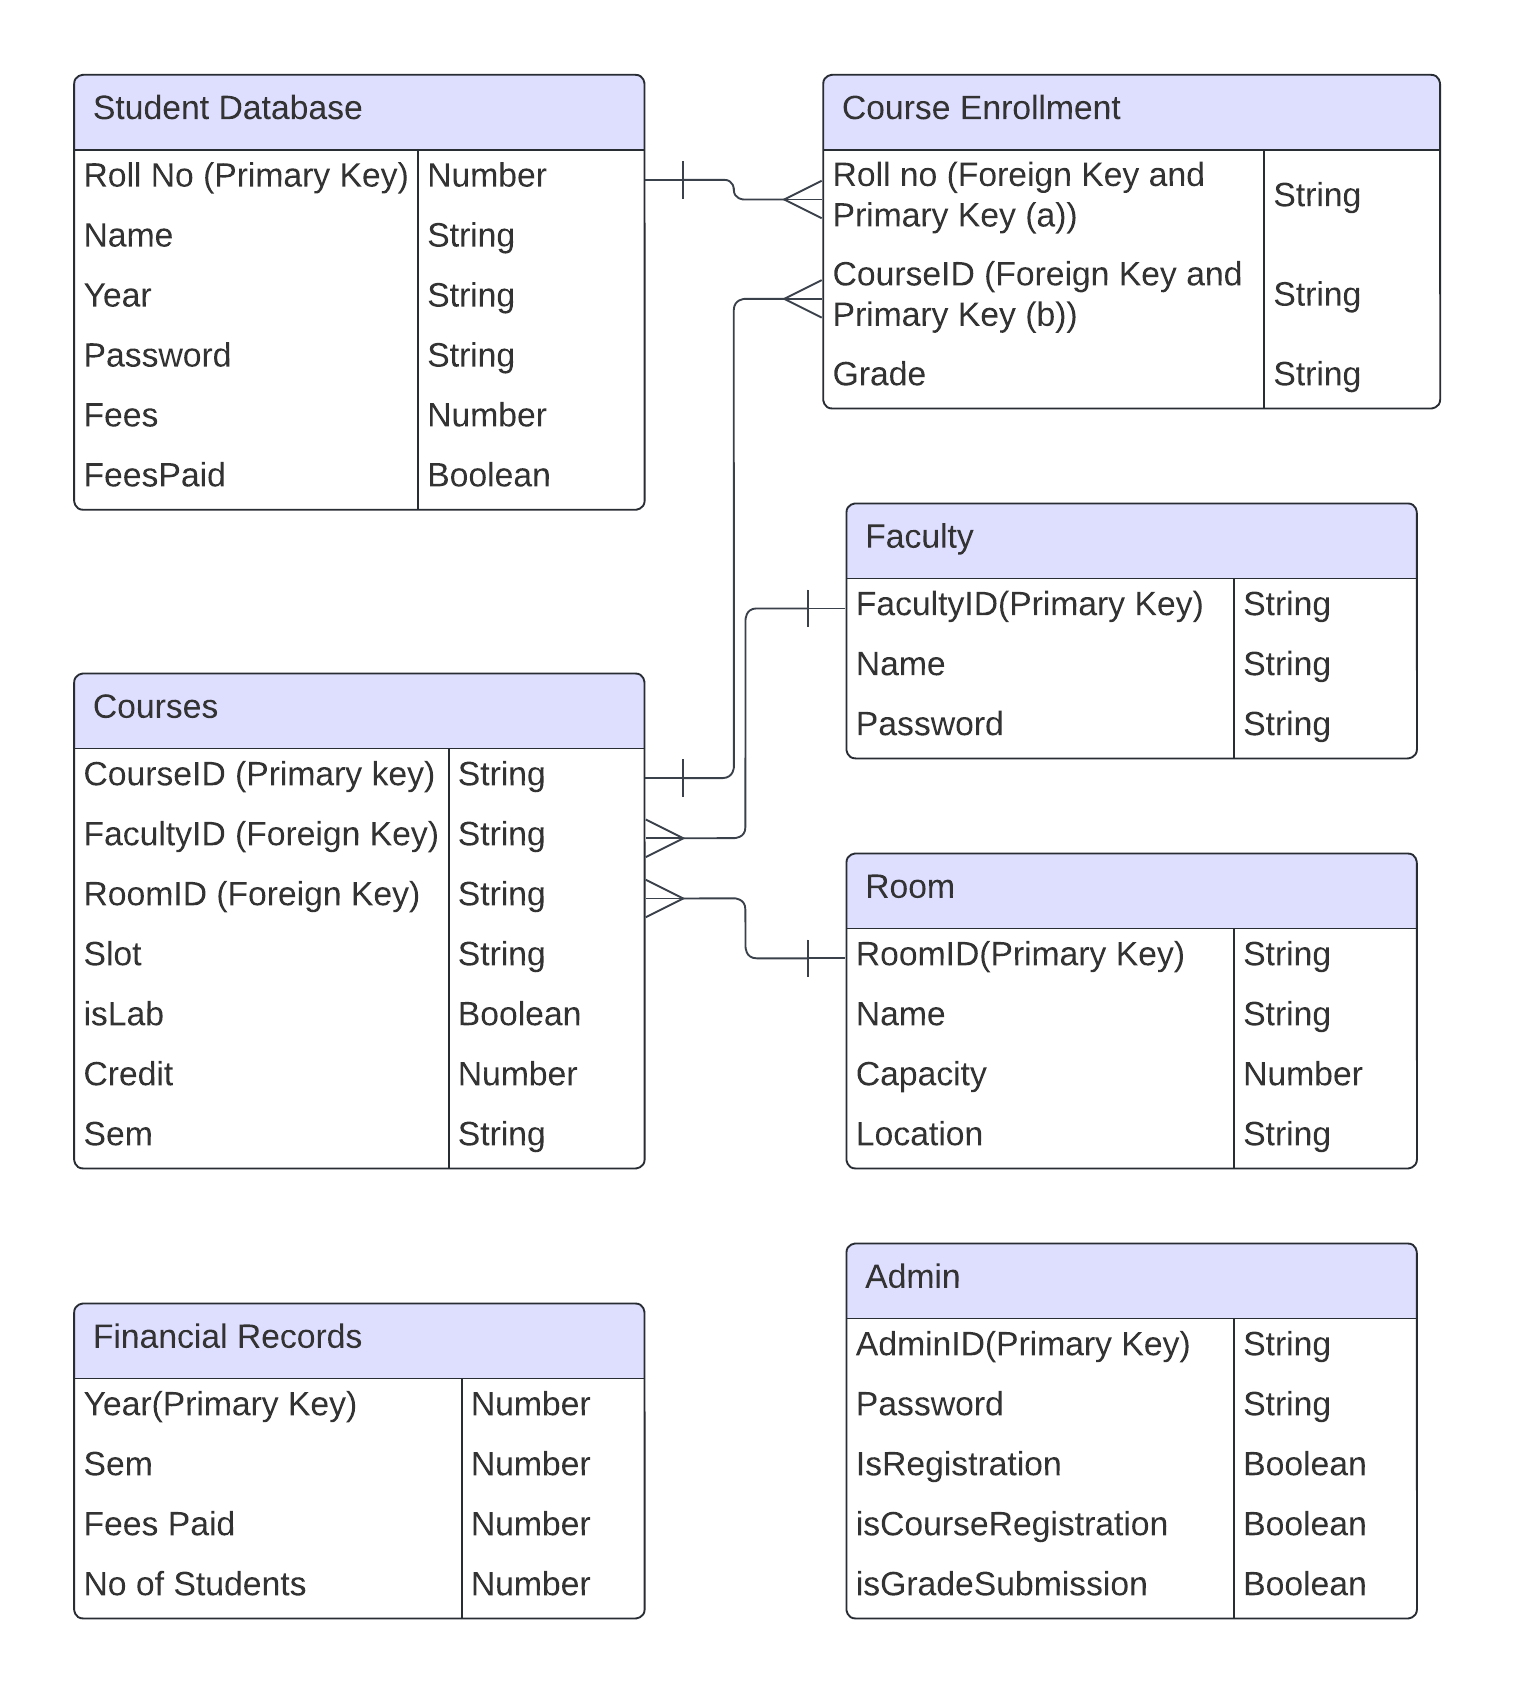
\includegraphics[scale=1.2]{ERDiagram.png} 
    \caption{\textbf{ER-Diagram}, Each Arrow represents a relation. A multiple-forked arrow represents Many relationships, whereas a single bar arrow represents one-one relationship.}
\end{figure}
    
    \subsection{Student Database}
        This database is used to store all information regarding students. The description of Each key is as follows:
        \begin{itemize}
        \item \textbf{Roll No:} Roll Number of student serves as Primary Key
        \item  \textbf{Name:} Name of Student
        \item  \textbf{Year:} Year Of Joining
        \item  \textbf{Password:} Password Used for authentication Purposes
        \item  \textbf{Fees:} Amount to be Paid By student
        \item  \textbf{FeesPaid:} Boolean to store if Fees paid or not
    \end{itemize}
    \subsection{Courses Database}
        This database is used to store all information regarding Courses.  The description of Each key is as follows:
        \begin{itemize}
        \item \textbf{CourseID:} Unique Identifier for Each Course. Serves as Primary key.
        \item  \textbf{FacultyID:} ID of faculty taking this course serves as a Foreign Key to faculty Table.
        \item  \textbf{RoomID:} ID of Room where this course will be held serves as a Foreign Key to Room Database.
        \item  \textbf{Slot:} Slot in which this course lectures are held. Assigned by TimeTable generator.
        \item  \textbf{isLab:} Boolean to store if It is a lab or not.
        \item  \textbf{Credit:} Credits of this course.
        \item  \textbf{Sem:} String to store sems in which this course is offered.
    \end{itemize}
    \subsection{Courses Taken Database}
        This database is used to store all information regarding which student took which Course. The pair (Roll No, CourseID) serves as a Primary Key. The description of Each key is as follows:
        \begin{itemize}
        \item \textbf{Roll No:} Roll No of student who has taken this course. Serves as Foreign Key to student Database.
        \item  \textbf{CourseID:} ID of Course taken. Serves as a Foreign Key to Courses Table.
        \item  \textbf{Grade:} Grade Received by student in that particular Course
    \end{itemize}
    \subsection{Faculty Database}
        This database is used to store all information regarding Faculties.  The description of Each key is as follows:
        \begin{itemize}
       \item \textbf{FacultyID:} Unique Identifier for Each Faculty. Serves as Primary key.
        \item  \textbf{Name:} Name of Faculty
        \item  \textbf{Password:} Password Used for authentication Purposes
    \end{itemize}
     \subsection{Room Database}
        This database is used to store all information regarding Rooms. The description of Each key is as follows:
        \begin{itemize}
       \item \textbf{RoomID:} Unique Identifier for Each Room. Serves as Primary key.
        \item  \textbf{Name:} Name of Room
        \item  \textbf{Capacity:} Capacity of Room
        \item  \textbf{Location:} Location of Room
    \end{itemize}
    \subsection{Admin Database}
        This database is used to store all information regarding Admin who controls the system. The description of Each key is as follows:
        \begin{itemize}
       \item \textbf{AdminID:} Unique Identifier for Admins. Serves as Primary key.
        \item  \textbf{Password:} Password Used for authentication Purposes
        \item  \textbf{isRegistration:} Boolean to start admission and Registration of new students.
        \item  \textbf{isCourseRegistration:} Boolean to start course Registration.
        \item  \textbf{isGradeSubmission:} Boolean to start Grade Submission.
    \end{itemize}
    \subsection{Financial Records}
        This database is used to store all information related to Finances. The description of Each key is as follows:
        \begin{itemize}
       \item \textbf{Year:} Year of Financial Record. Serves as Primary key.
        \item  \textbf{Sem:} Semester
        \item  \textbf{FeesPaid:} How much Fees is paid.
        \item  \textbf{No of Students:} Number of Registered Students.
    \end{itemize}
    
\section{Feature Enhancement}
The following points outline the feature enhancements that can be applied to the software in later stages:
\begin{itemize}
    \item Extend the system to support a broader range of courses and include students from other programs, not limited to B.Tech CSE.
    \item Allow faculties to provide new courses themselves and approve/reject the enrollment of students.
    \item Allow for more flexibility in defining the criteria for student distinction, considering tutorial and lab groups.
    \item Provide administrators with the ability to set variable durations for lectures and labs.
    \item Extend the system to support multiple faculty members for a single course.
    \item Implement a system that allows students to request changes to their enrolled courses during the semester under certain conditions.
    \item Develop a dedicated interface for administrators to manage rooms, including scheduling, capacity planning, and maintenance information.
\end{itemize}
        
\section{User Interface}
(Shivam Agrawal)
	The user interface for this software can be developed using \texttt{Visual Basic}. The following are the tentative list of toolbox components needed for the basic implementation (without any feature enhancement):
    \begin{itemize}
        \item \textbf{Text Box:} sdfeerererererer
        \item And so on....
    \end{itemize}

    \subsection{Basic Design}
    This is the tentative basic design of the user interface which is to be designed in \textbf{Visual Basic} using the components listed above:
    \begin{figure}[H]
        \centering
        \begin{subfigure}[b]{0.45\linewidth}
            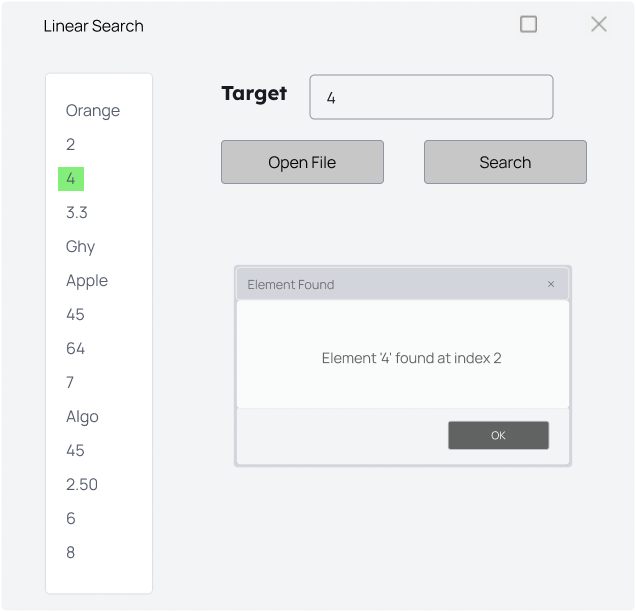
\includegraphics[width=\linewidth]{Prototype.png} 
            \caption{Message box output when element is found.}
            \label{fig:sub1}
        \end{subfigure}
        \hfill
        \begin{subfigure}[b]{0.45\linewidth}
            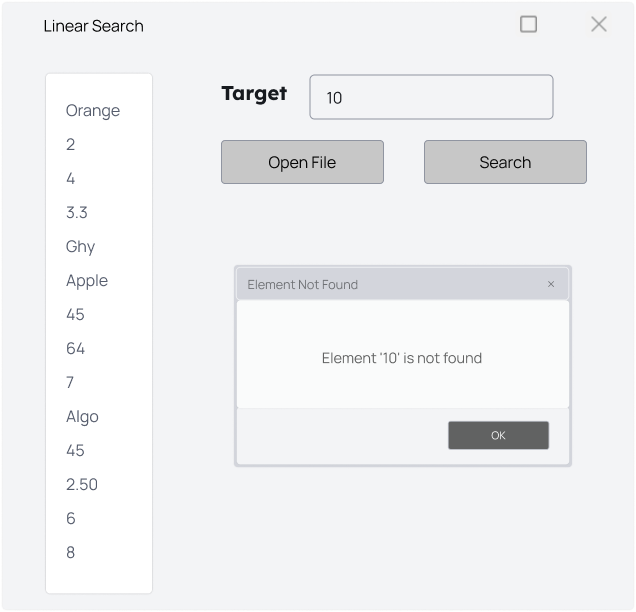
\includegraphics[width=\linewidth]{Prototype-2.png}
            \caption{Message box output when element is not found.}
            \label{fig:sub2}
        \end{subfigure}
        \caption{Basic design of the software application}
        \label{fig:overall}
    \end{figure}
\subsection{Subsections}
\end{document}
